We identify points with elements of $\mathbb{R}^2$. Concretely,~\lstinline|abbrev Point := EuclideanSpace ℝ (Fin 2)|.
The next step is to define what it means for a $k$-gon to be \emph{empty} (with respect to a set of points) and \emph{convex}, which we do in terms of \textsf{mathlib} primitives.

\begin{lstlisting}
/-- `EmptyShapeIn S P' means that `S' carves out an empty shape in `P':
the convex hull of `S' contains no point of `P' other than those already in `S'. -/
def EmptyShapeIn (S P : Set Point) : Prop :=
    ∀ p ∈ P \ S, p ∉ convexHull ℝ S

/-- `ConvexPoints S' means that `S' consists of extremal points of its convex hull,
i.e., the point set encloses a convex polygon. -/
def ConvexPoints (S : Set Point) : Prop :=
    ∀ a ∈ S, a ∉ convexHull ℝ (S \ {a})

def ConvexEmptyIn (S P : Set Point) : Prop :=
    ConvexPoints S ∧ EmptyShapeIn S P

def HasEmptyKGon (k : Nat) (S : Set Point) : Prop :=
    ∃ s : Finset Point, s.card = k ∧ ↑s ⊆ S ∧ ConvexEmptyIn s S
\end{lstlisting}

Let \lstinline|ListInGenPos| be a predicate that states that a list of points is in \emph{general position}, i.e., no three points lie on a common line (made precise in~\Cref{sec:triple-orientations}).
With this we can already state the main theorem of our paper.

\begin{lstlisting}
theorem hole_6_theorem (pts : List Point) (gp : ListInGenPos pts)
    (h : pts.length ≥ 30) : HasEmptyKGon 6 pts.toFinset
\end{lstlisting}

At the root  of the encoding of Heule and Scheucher is the idea that the~\lstinline|ConvexEmptyIn| predicate can be determined by analyzing only triangles. In particular, that a set $s$ of $k$ points in a pointset $S$ form an empty convex $k$-gon if and only if all the ${k \choose 3}$ triangles induced by vertices in $s$ are empty with respect to $S$. This is discussed informally in~\cite[Section 3, Eq.~4]{emptyHexagonNumber}.
Concretely, we prove the following theorem:
\begin{lstlisting}
theorem ConvexEmptyIn.iff_triangles {s : Finset Point} {S : Set Point}
    (sS : ↑s ⊆ S) (sz : 3 ≤ s.card) :
    ConvexEmptyIn s S ↔
    ∀ (t : Finset Point), t.card = 3 → t ⊆ s → ConvexEmptyIn t S
\end{lstlisting}
\begin{figure}
    \centering
    \begin{subfigure}{0.45\textwidth}
        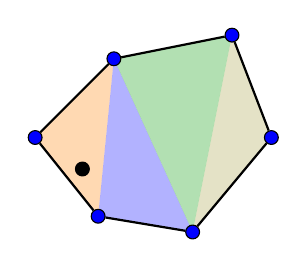
\begin{tikzpicture}
        \coordinate (a) at (0,0);
        \coordinate (b) at (1, 1);
        \coordinate (c) at (2.5, 1.3);
        \coordinate (d) at (3, 0);
        \coordinate (e) at (0.8, -1);
        \coordinate (f) at (2, -1.2);

        \fill[orange, opacity=0.3] (a) -- (b) -- (e) -- (a) -- cycle;
        \fill[blue, opacity=0.3] (b) -- (f) -- (e) -- (b) -- cycle;
        \fill[green!60!black, opacity=0.3] (b) -- (c) -- (f) -- (b) -- cycle;
        \fill[yellow!60!black, opacity=0.3] (c) -- (d) -- (f) -- (c) -- cycle;

        \node[draw, circle, black, fill=blue, inner sep=0pt, minimum size=5pt] (pA) at (0, 0) {};
        \node[draw, circle, black, fill=blue, inner sep=0pt, minimum size=5pt] (pB) at (1, 1) {};
        \node[draw, circle, black, fill=blue, inner sep=0pt, minimum size=5pt] (pC) at (2.5, 1.3) {};
        \node[draw, circle, black, fill=blue, inner sep=0pt, minimum size=5pt] (pD) at (3, 0) {};
        \node[draw, circle, black, fill=blue, inner sep=0pt, minimum size=5pt] (pE) at (0.8, -1) {};
        \node[draw, circle, black, fill=blue, inner sep=0pt, minimum size=5pt] (pF) at (2, -1.2) {};

        \node[draw, circle, black, fill=black, inner sep=0pt, minimum size=5pt] (pG) at (0.6, -0.4) {};


        \draw[thick] (pA) -- (pB) -- (pC) -- (pD) -- (pF) -- (pE) -- (pA);
        % \draw[dashed, thick, red] (pA) -- (pB) -- (pE) -- (pA);
        % \draw[dashed, thick, blue] (pB) -- (pF) -- (pE) -- (pB);
        % \draw[dashed, thick, green!60!black] (pB) -- (pC) -- (pF) -- (pB);


        \end{tikzpicture}
        \caption{}
    \end{subfigure}
    \begin{subfigure}{0.45\textwidth}
        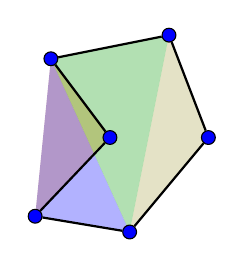
\begin{tikzpicture}
            \coordinate (a) at (1.75,0);
            \coordinate (b) at (1, 1);
            \coordinate (c) at (2.5, 1.3);
            \coordinate (d) at (3, 0);
            \coordinate (e) at (0.8, -1);
            \coordinate (f) at (2, -1.2);

            \fill[orange, opacity=0.3] (a) -- (b) -- (e) -- (a) -- cycle;
            \fill[blue, opacity=0.3] (b) -- (f) -- (e) -- (b) -- cycle;
            \fill[green!60!black, opacity=0.3] (b) -- (c) -- (f) -- (b) -- cycle;
            \fill[yellow!60!black, opacity=0.3] (c) -- (d) -- (f) -- (c) -- cycle;

            \node[draw, circle, black, fill=blue, inner sep=0pt, minimum size=5pt] (pA) at (1.75, 0) {};
            \node[draw, circle, black, fill=blue, inner sep=0pt, minimum size=5pt] (pB) at (1, 1) {};
            \node[draw, circle, black, fill=blue, inner sep=0pt, minimum size=5pt] (pC) at (2.5, 1.3) {};
            \node[draw, circle, black, fill=blue, inner sep=0pt, minimum size=5pt] (pD) at (3, 0) {};
            \node[draw, circle, black, fill=blue, inner sep=0pt, minimum size=5pt] (pE) at (0.8, -1) {};
            \node[draw, circle, black, fill=blue, inner sep=0pt, minimum size=5pt] (pF) at (2, -1.2) {};

            % \node[draw, circle, black, fill=black, inner sep=0pt, minimum size=5pt] (pG) at (0.6, -0.4) {};


            \draw[thick] (pA) -- (pB) -- (pC) -- (pD) -- (pF) -- (pE) -- (pA);
            % \draw[dashed, thick, red] (pA) -- (pB) -- (pE) -- (pA);
            % \draw[dashed, thick, blue] (pB) -- (pF) -- (pE) -- (pB);
            % \draw[dashed, thick, green!60!black] (pB) -- (pC) -- (pF) -- (pB);


        \end{tikzpicture}
        \caption{}
    \end{subfigure}
    \caption{Illustration of the proof for \lstinline|ConvexEmptyIn.iff_triangles|. The left subfigure shows how a point inside the polygon implies the point is inside one of the triangles of triangulation of its convex hull. The right subfigure shows how non-convexity implies one of the vertices of the polygon will be inside one of the triangles of the convex hull partition.}\label{fig:triangulation}
\end{figure}

\begin{proof}[Proof sketch]
    We first prove a simple monotonicity lemma: if $\textsf{ConvexPoints}(s)$, then $\textsf{ConvexPoints}(s')$ for every $s' \subseteq s$, and similarly $\textsf{EmptyShapeIn}(s, S) \Rightarrow \textsf{EmptyShapeIn}(s', S)$ for every set of points $S$.
    By instantiating this monotonicity lemma over all subsets $t \subseteq s$ with $|t| = 3$ we get the forward direction of the theorem.
    For the backward direction it is easier to reason contrapositively: if the~$\textsf{ConvexPoints}$ predicate does not hold of $s$, or if $s$ is not empty w.r.t.~$S$, then we want to show that there is a triangle $t \subseteq s$ that is also not empty w.r.t.~$S$. To see this, let $H$ be the convex hull of $s$, and then by Carath\'eodory's theorem (cf. \lstinline|theorem convexHull_eq_union| from \textsf{mathlib}), every point in $H$ is a convex combination of at most $3$ points in $s$, and consequently, of exactly $3$ points in $s$.
    If $s$ is non-empty w.r.t.~$S$, then there is a point $p \in S \setminus s$ that belongs to $H$, and by Carath\'eodory, $p$ is a convex combination of $3$ points in $s \setminus \{a\}$, and thus lies inside a triangle $t \subseteq s$ (\Cref{fig:triangulation-a}). If $s$ does not hold $\textsf{ConvexPoints}$, then there is a point $a \in s$ such that $a \in \textsf{convexHull}(s \setminus \{a\})$, and by Carath\'eodory again, $a$ is a convex combination of $3$ points in $s$, and thus lies inside a triangle $t \subseteq s \setminus \{a\}$ (\Cref{fig:triangulation-b}).
%     The
%     The forward direction is easy to see, as triangles are always convex, and if $s$ is empty w.r.t.~$S$, then so are the triangles induced by vertices of $s$.
%     Let $T = \{t_1, \ldots, t_{{k \choose 3}}\}$ be all the triangles induced by vertices of $s$.
%    For the backward direction we will need a \emph{triangulation lemma} stating that the convex hull of $s$ can be partitioned into triangles $P = \{t_i, \ldots, t_j\}$, and $P \subseteq T$.
%     To see that if every $t \in T$ is empty w.r.t. $S$ then $s$ is also empty w.r.t. $S$ we can use the contrapositive statement.
    %  Indeed, assume $s$ is not empty w.r.t. $S$, there is a point $p \in S \setminus s$ that lies inside the convex hull of $s$. Because $P$ is a partition of the convex hull of $s$, point $p$ must be inside some $t \in P \subseteq T$.
    %  To see convexity, we can reason contrapositively again. If $s$ is not convex, then there is a point $p \in s$ that lies inside the convex hull of $s$, and thus lies inside a triangle $t \in P$.
\end{proof}

In the next section,
we show how to encode which triangles (and, by the above theorem, which $k$-holes) are empty in a pointset with boolean variables.